% !TeX root = ../thuthesis-example.tex

\chapter{实验结果}
\section{SP-SOLD2网络性能实验}
为了评估SP-SOLD2网络的性能,本工作在Hpatches\cite{balntas2017hpatches}数据集上测试了点特征的匹配性能,在Wireframe\cite{huang2018learning}数据集上测试了线特征的提取效果。
\subsection{点特征匹配测试结果}
\begin{figure}
  \centering
  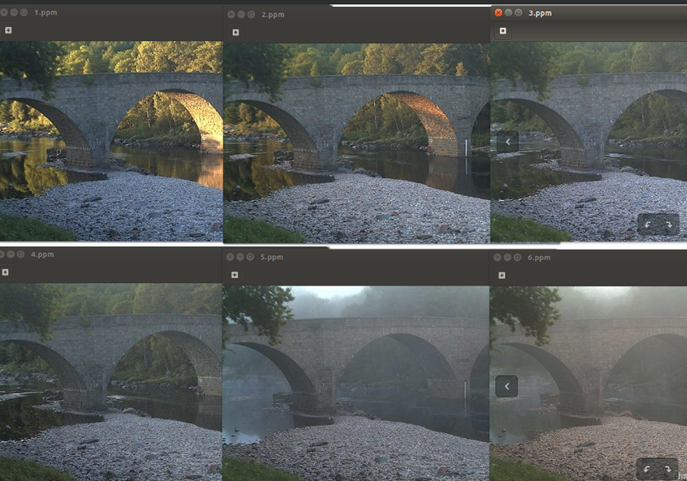
\includegraphics[width = 0.85\textwidth]{Hpatch.png}
  \label{fig_hpatch}
  \caption{Hpatches数据集中的图像序列}
\end{figure}

Hpatches数据集包含了108个图像序列,每个图像序列包括1张参考图像和5张在不同照明条件下/不同视角下拍摄的目标图像。如图\ref{fig_hpatch}所示,每个序列中包括的6张图像形成了5对图像对,并均给出了真实的单应性估计用于图像配准。实验的评估指标(MMA@n)是在误差阈值为n个像素点时,Hpatches数据集中每一对图片的特征点匹配的平均正确率。

如图\ref{fig_hpatch_res}和表\ref{tab_hpatch_res}所示,相比于目前的一些主流点特征描述子提取网络,我们的算法获得了更高的匹配精度。而相对于作为母方法的Superpoint网络,SP-SOLD2在加入线特征分支后也仍然保持了点特征部分的性能,在光照变化场景下甚至有更好的匹配效果。
\begin{figure}
  \centering
  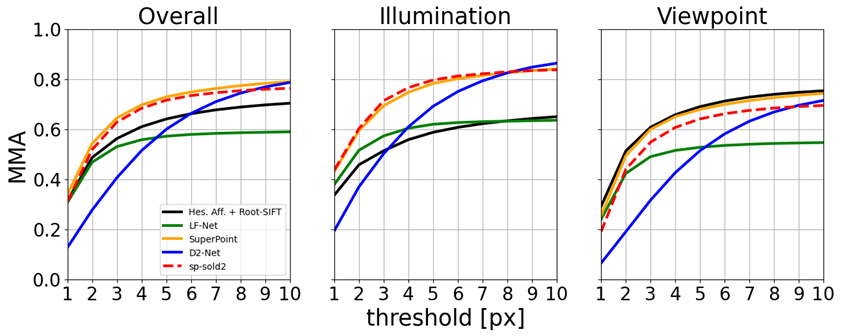
\includegraphics[width = 0.85\textwidth]{hpatch_res.png}
  \caption{点特征匹配测试结果}
  \label{fig_hpatch_res}
\end{figure}
\begin{table}[!ht]
  \centering
  \begin{tabular}{|c|c|c|c|}
  \hline
      Algorithm & MMA@1 & MMA@3 & MMA@5 \\ \hline
      LF-Net & 0.31 & 0.53 & 0.57 \\ \hline
      D2-Net & 0.12 & 0.40 & 0.60 \\ \hline
      SuperPoint & 0.33 & 0.64 & 0.73 \\ \hline
      Ours & 0.31 & 0.61 & 0.71 \\ \hline
  \end{tabular}
  \caption{点特征匹配测试结果}
  \label{tab_hpatch_res}
\end{table}

\subsection{线特征匹配测试结果}
Wireframe数据集用作直线段检测数据集,包含5462张场景图像,其中5000张图像用于训练,其余462张图像用于测试,如图\ref{fig_wireframe}所示。在Wireframe数据集下本工作测试了两个指标:线段检测重复性(Rep)和线段定位准确率(Loc)。
\begin{figure}
  \centering
  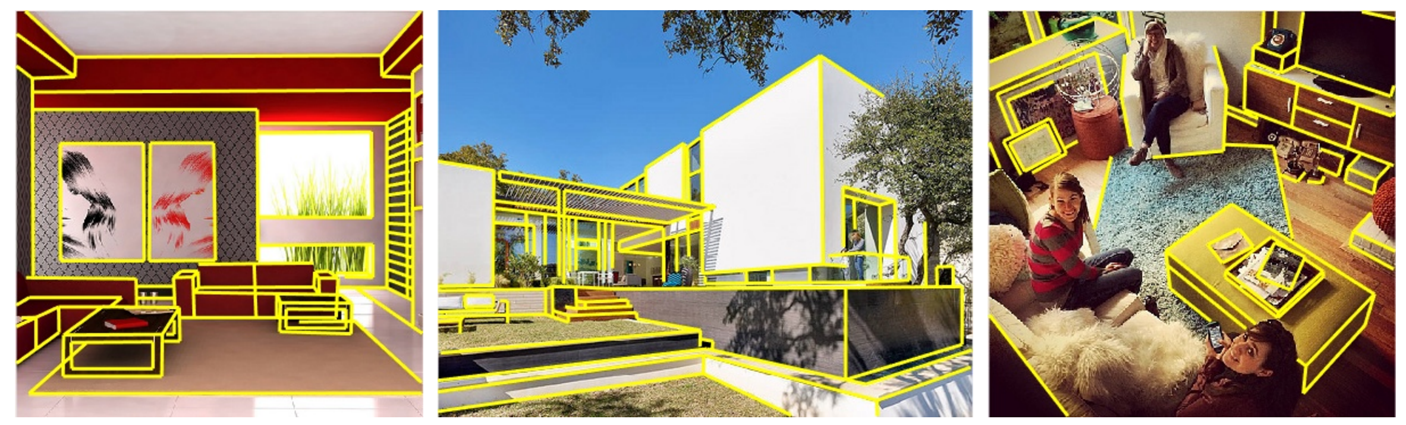
\includegraphics[width = 0.85\textwidth]{wireframe.png}
  \caption{Wireframe数据集中的图像}
  \label{fig_wireframe}
\end{figure}

从测试结果表\ref{tab_lineres}可见,相对于当前主流的神经网络线提取算法,SP-SOLD2网络在检测可重复性和定位准确度上都有更好的表现;而相对于其母方法SOLD2网络,SP-SOLD2由于缩减了网络规模,加入了点特征分支,故而性能有所下降,不过相对于实时性能的提升,这部分精度损失是可以容忍的。
\begin{table}[!ht]
  \centering
  \begin{tabular}{|c|c|c|}
  \hline
      Algorithm & Rep-5 & Loc-5 \\ \hline
      LSD & 0.358 & 2.079 \\ \hline
      SOLD2 & 0.525 & 2.009 \\ \hline
      LCNN & 0.434 & 2.589 \\ \hline
      TP-LSD & 0.358 & 3.220 \\ \hline
      Ours & 0.440 & 2.49 \\ \hline
  \end{tabular}
  \caption{线特征匹配测试结果}
  \label{tab_lineres}
\end{table}

\section{点线VIO系统性能实验}
本项目在Euroc数据集\cite{burri2016euroc}上完成了验证。Euroc数据集是微型无人机 (MAV) 上收集的视觉惯性数据集,采集到的数据包含视觉图像(尺寸)、IMU 测量数据以及毫米级的运动估计和地图结构,采集场景包括大学机房室内场景和普通房间室内场景,如图\ref{fig_euroc}所示。数据集根据场景类型、飞行轨迹和光照条件分为了不同难度的多个用例。
\begin{figure}
  \centering
  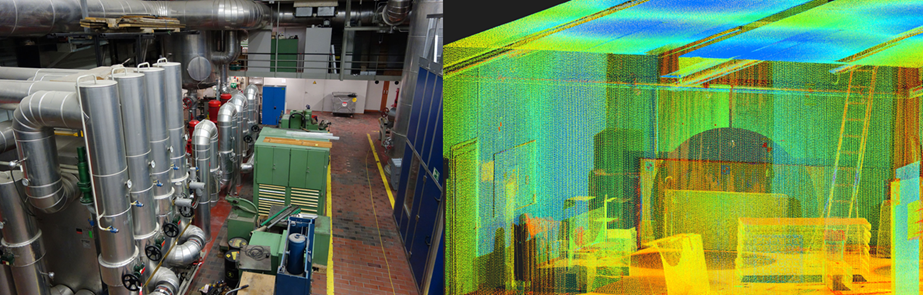
\includegraphics[width = 0.85\textwidth]{euroc.png}
  \caption{Euroc数据集中的图像}
  \label{fig_euroc}
\end{figure}

为了测试点线VIO系统在室内场景中的定位精度和实时性能,本工作选取了Euroc数据集中较困难的几个场景,测试了轨迹估计的均方根误差(RMSE)并和原方法PL-VINS进行了对比,如表\ref{tab_euroc_res}所示。
\begin{table}[!ht]
  \centering
  \begin{tabular}{|c|c|c|}
  \hline
      Dataset & PL-VINS & NN-PL-VIO \\ \hline
      MH-04-difficult & 0.270 & 0.200 \\ \hline
      MH-05-difficult & 0.272 & 0.157 \\ \hline
      V1-02-medium & 0.105 & 0.105 \\ \hline
      V1-03-difficult & 0.156 & 0.054 \\ \hline
      V2-03-difficult & 0.237 & 0.129 \\ \hline
      Mean & 0.208 & 0.129 \\ \hline
  \end{tabular}
  \caption{NN-PL-VIO测试结果}
  \label{tab_euroc_res}
\end{table}

同时本项目还对系统运算时间进行了测试分析,结果如表\ref{tab_inf_time}所示。
\begin{table}[!ht]
  \centering
  \begin{tabular}{|c|c|c|c|c|c|c|}
  \hline
      ~ & Inference & Point Reprocess & Line Reprocess & Point Match & Line Match & Backend \\ \hline
      Time (ms) & 8 & 11 & 70 & 5 & 32 & 90 \\ \hline
  \end{tabular}
  \caption{运算时间测试结果}
  \label{tab_inf_time}
\end{table}

可见,采用SP-SOLD2网络作为前端,在开源数据集上轨迹估计精度将相比于原PL-VINS方法提升~38\%;而通过速度优化,本工作将最耗时的点、线特征后处理部分分别提升了12x和15x,使得整个系统的处理帧率达到11.1fps,初步满足实时性需求。

\section{总结与讨论}
针对现有点线联合VIO系统中缺少支持神经网络方法框架的问题,本课题基于PL-VINS框架建立了一个前端自定义的NN-PL-VINS框架,该框架支持用户自定义前端的点线提取和匹配方法,便于用户在不同场景下选择适合的方法以获得更佳的性能。
针对现有点线联合VIO系统中线检测和参数化耗时高的问题,本课题构造了一个点线联合推理网络SP-SOLD2,该网络可以通过一次推理得到点特征和线特征的提取结果以及对应的描述子,并且通过后处理的优化以及pipeline构建,在Euroc数据集中,此网络可以在NN-PL-VINS框架中取得相对现有工作更好的精度效果(~38\%的精度提升)和较好的的实时性能(11.1fps)。
本课题建立的实时性点线联合VIO系统在室内数据集上有较佳的表现,但是对于高景深的室外数据集表现欠佳。为了解决这个问题,未来工作还可以尝试用室外数据集对自监督网络进行fine-tune以达到更好的提取效果,也可以继续探究同时适配于室内外的嵌入式实时VIO系统。
